\documentclass[paperwidth=160cm,paperheight=100cm,landscape,fontscale=0.3010]{baposter}
%Dortes fontscale: 0.2941
\usepackage{lipsum} 
%841mm x 1189mm
\usepackage[font=small,labelfont=bf,hypcap=false]{caption} % Required for specifying captions to tables and figures
%\usepackage{cite}
\usepackage{booktabs} % Horizontal rules in tables
\usepackage{relsize} % Used for making text smaller in some places
%\usepackage[urlcolor  = blue]{hyperref}
%\graphicspath{{figures/}} % Directory in which figures are stored
\usepackage{multicol}
%\usepackage[style=ieee]{biblatex}
%\addbibresource{bib.bib}
\usepackage[utf8]{inputenc} 
%\usepackage{hyperref}
\usepackage{placeins}
\usepackage{epstopdf}
\usepackage{subcaption}
\usepackage[]{graphicx}
\usepackage{natbib}
\usepackage{times}

\usepackage[utf8]{inputenc}
\usepackage{fourier} 
\usepackage{array}
\usepackage{makecell}

\bibliographystyle{abbrvnat}

\selectcolormodel{RGB} %<-- Add colour model defintion
\definecolor{bordercol}{RGB}{255,255,255}%{33,26,82} % Border color of content boxes
\definecolor{headercol1}{RGB}{255,255,255}%{33,26,82} % Background color for the header in the content boxes (left side)
%\definecolor{headercol2}{RGB}{5,2,82} % Background color for the header in the content boxes (right side)
\definecolor{headerfontcol}{RGB}{0,0,0}%{255,255,255} % Text color for the header text in the content boxes
\definecolor{boxcolor}{RGB}{255,255,255} % Background color for the content in the content boxes

\begin{document}
\graphicspath{{Pictures/}}
\background{ % Set the background to an image (background.pdf)

}

\begin{poster}{
grid=false,
headerheight=0.14\textheight,
borderColor=bordercol, % Border color of content boxes
headerColorOne=headercol1, % Background color for the header in the content boxes (left side)
%headerColorTwo=headercol2, % Background color for the header in the content boxes (right side)
headerFontColor=headerfontcol, % Text color for the header text in the content boxes
boxColorOne=boxcolor, % Background color for the content in the content boxes
headershape=rectangle, % Specify the rounded corner in the content box headers
headershade=plain,
headerfont=\Large\sf\bf, % Font modifiers for the text in the content box headers
textborder=rectangle,
background=user,
headerborder=open, % Change to closed for a line under the content box headers
boxshade=plain,
eyecatcher=true
}
%
%----------------------------------------------------------------------------------------
%	TITLE AND AUTHOR NAME
%----------------------------------------------------------------------------------------
%
%\vspace{2em}
% Eye Catcher Images to go left of your title.
{

\includegraphics[height=0.10\textheight]{aau_logo_new.eps}
} %will not show if put eyecatcher=false
% Title
{\vspace{2pt}
Subjective Experience of Interacting with a Social Robot at a Danish Airport}
% Author
{
\vspace{3pt}
\normalsize{\textbf{Andreas Kornmaaler Hansen, Emil Bonnerup, Juliane Nilsson, Lucca Julie Nellemann \& Sara Nielsen}\\
Psychology Engineering - 17gr782 - Fall 2017 - School of Information and Communication Technology\\ Aalborg University, Aalborg, Denmark\\ }
$\{$akha14, ebonne14, jnils12, ljne14, snie14$\}$@student.aau.dk\\
}
{

\includegraphics[height=0.10\textheight]{aau_logo_new.eps}
}

%----------------------------------------------------------------------------------------
%	INTRODUCTION
%----------------------------------------------------------------------------------------
\headerbox{Introduction}
{name=introduction,column=0,row=0, span=1}
{\parskip 5pt   
This study originates from a social robot research project at Aalborg University with the aim of developing and implementing robots in a variety of contexts. This raises questions on how social robots should behave and which variables in a social robot is important. When important variables are eliciteted scales can be developed from these variables which can be use to test a social robot. The study consists of two tests, one where variables are elicitated and one where the scales are used to evaluate the robot, so possible correlation can be detected.  
}

\headerbox{Methods}
{name=method,span=1,column=0,below=introduction, span=1}
{\parskip 5pt 
To investigate which variables are important when interacting with social robots and to check for correlation on scales designed based on these variabels two tests are set up in Aalborg Airport (AAL). Both tests was conducted on Danish Travellers who interacted with a \textit{Double} robot shown on figure 1. In the first test subjects was asked to participate in a semi-structured interview about their first impressions after the interaction and in the second test subjects were asked to rate their interactions on the developed scales. The \textit{Double} robot was remotely controlled via a computer and a present controller. On the screen a developed wireframe to help with wayfinding in AAL was presented. 
\vspace{-10pt}  

\begin{center}
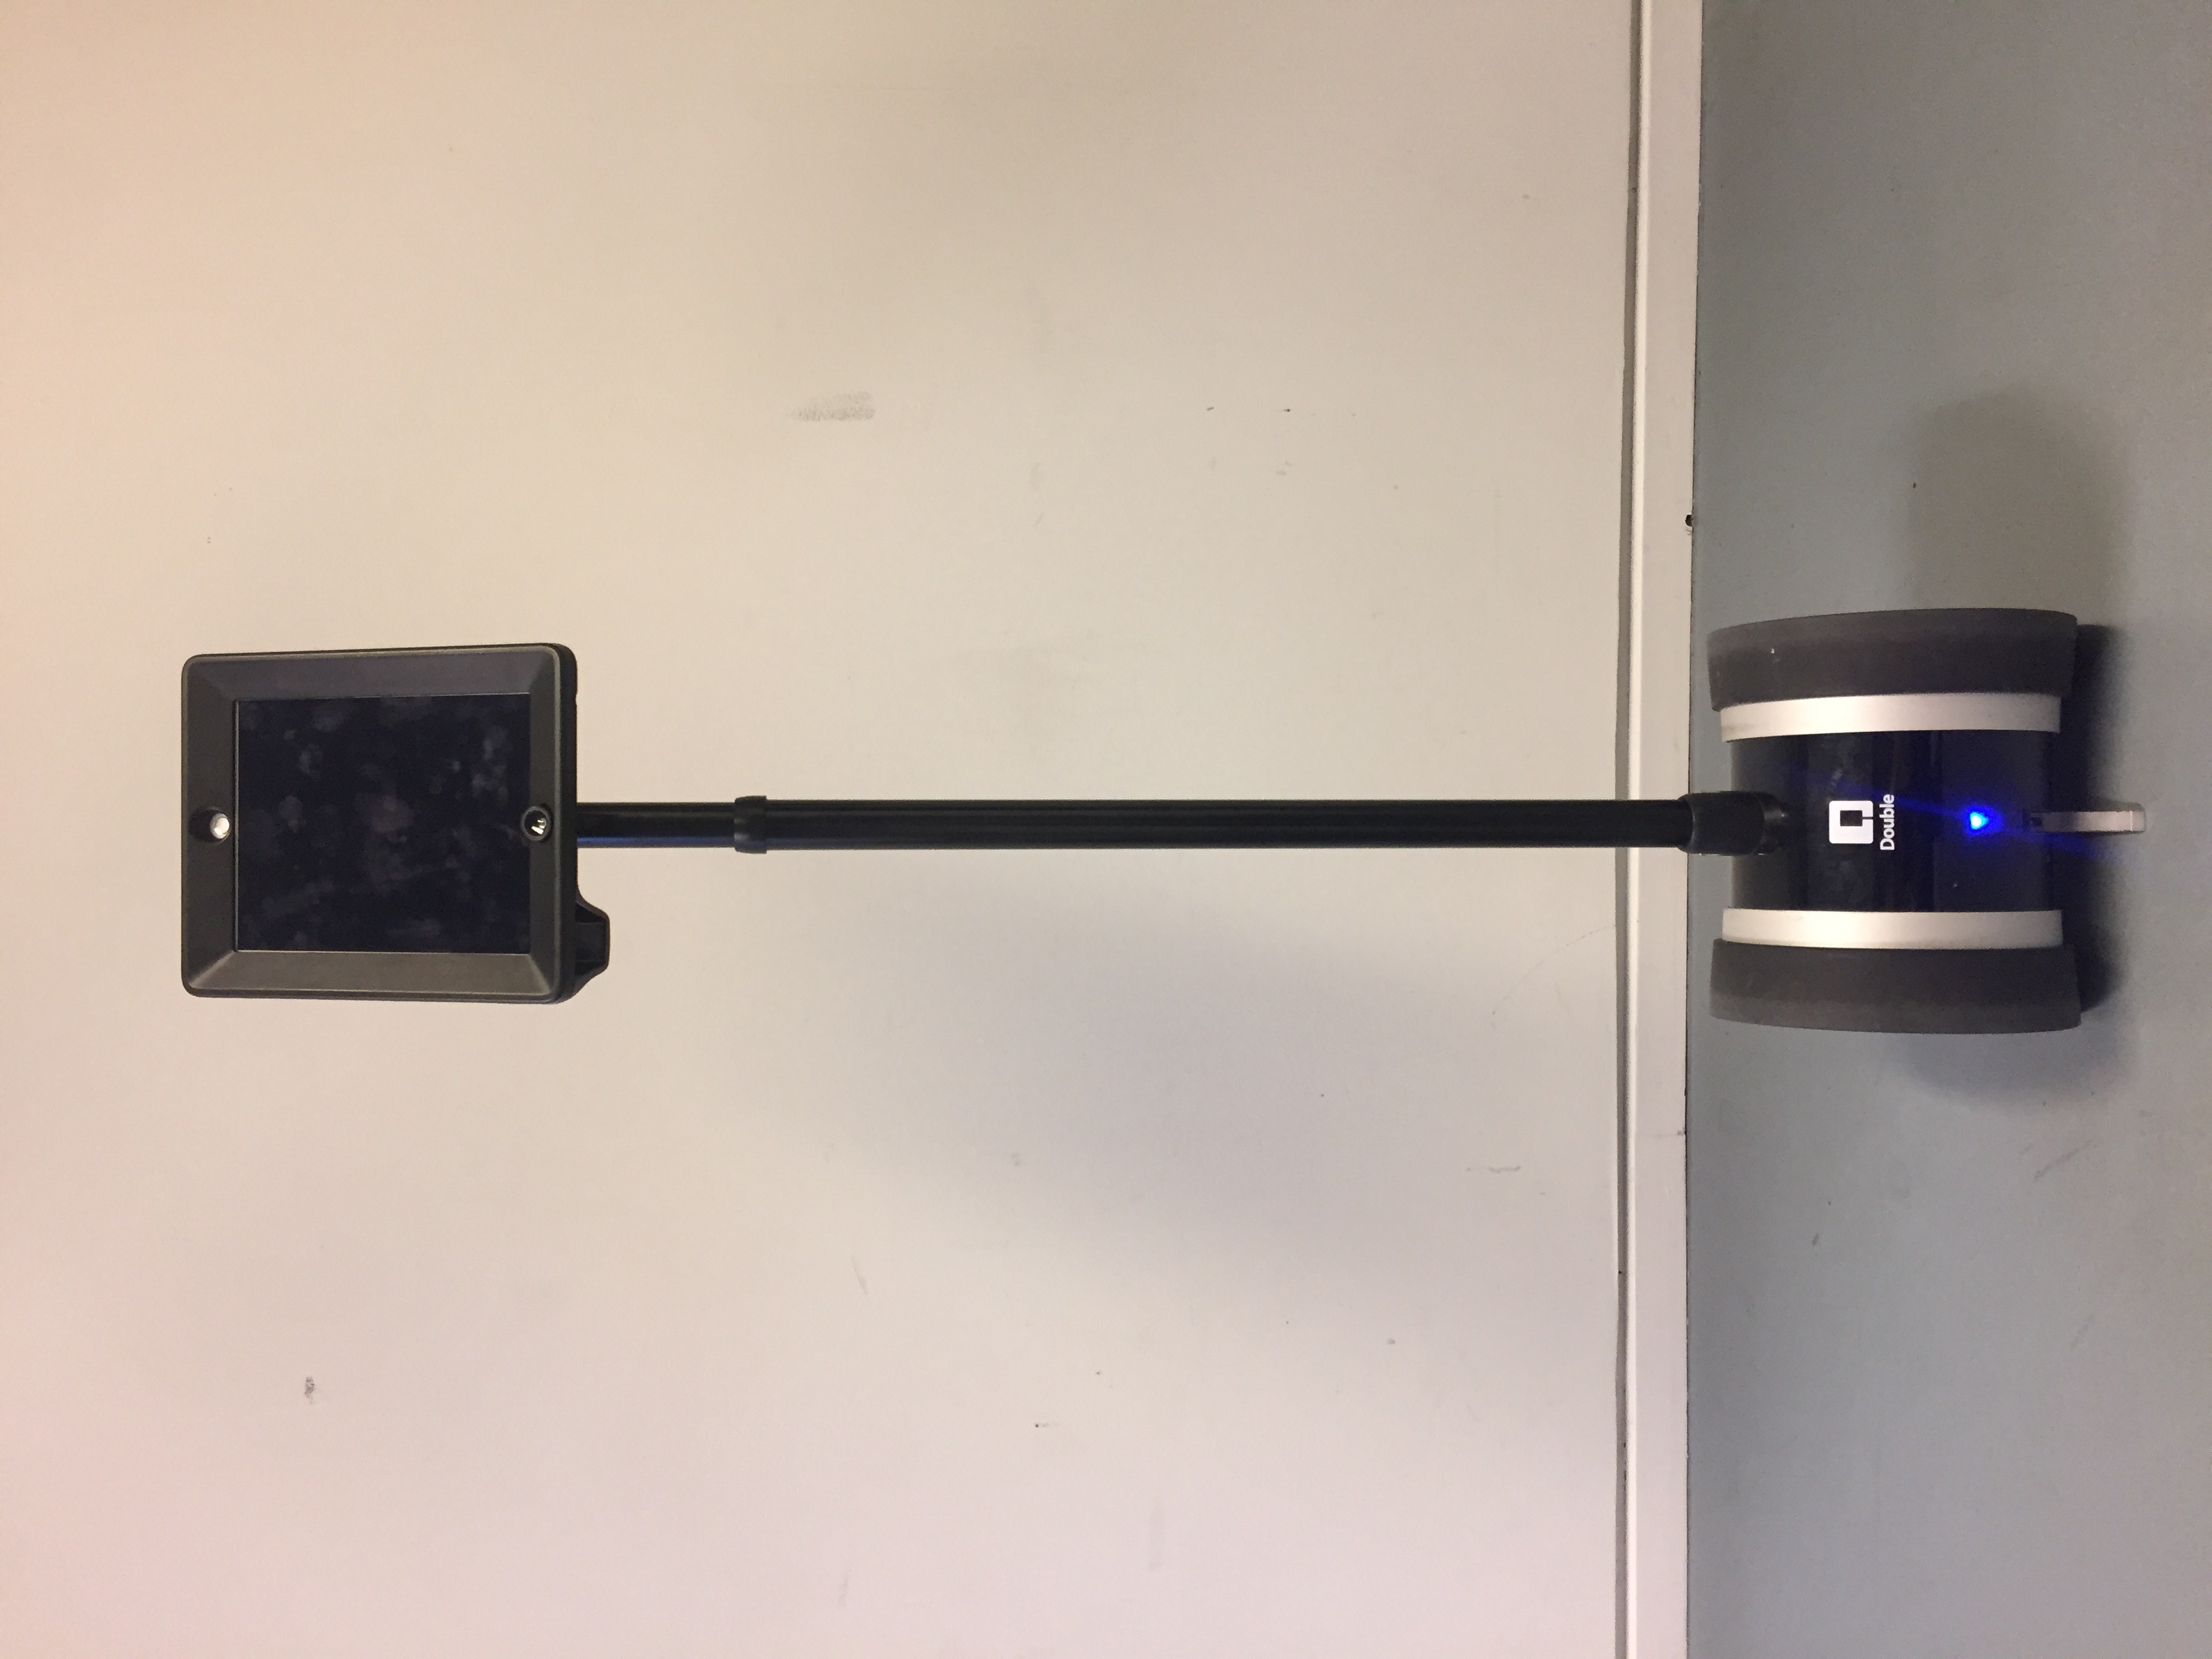
\includegraphics[width=0.30\linewidth]{ModificeretDoubleFront.eps}
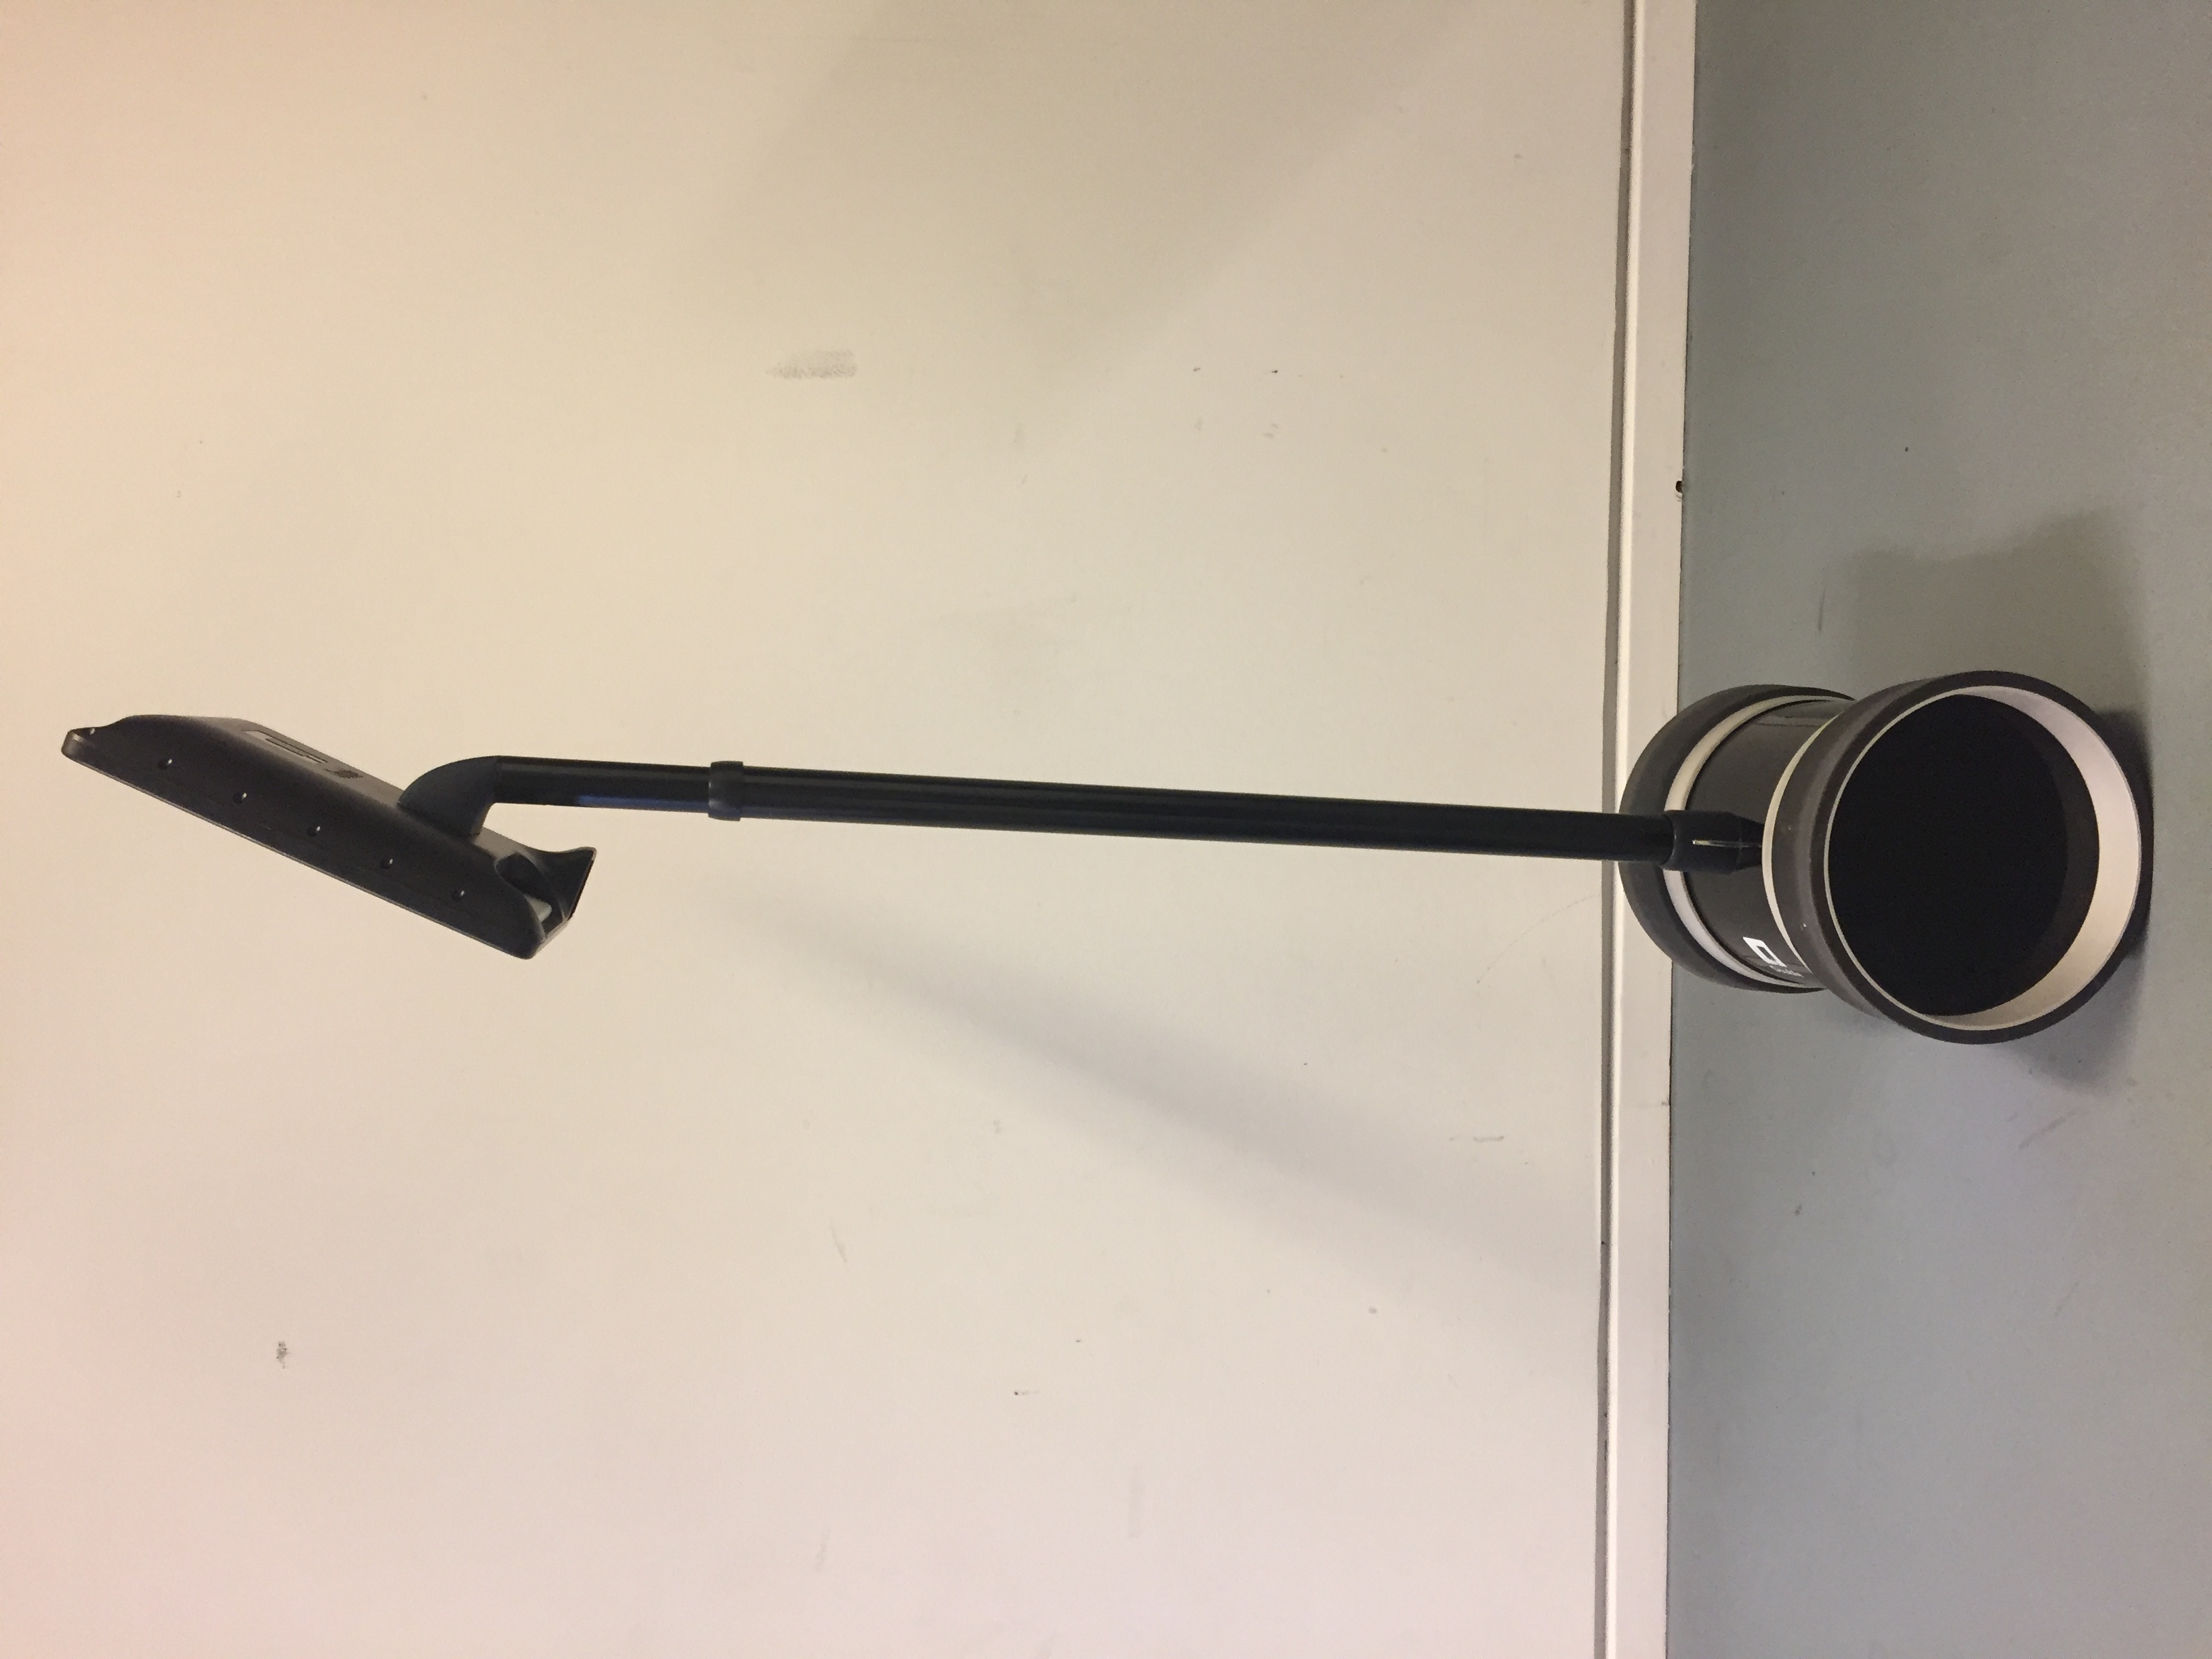
\includegraphics[width=0.30\linewidth]{ModificeretDoubleSide.eps}

\textbf{Figure~1. }\textit{Double}'s front and profile.
\end{center}
\vspace{-10pt}  

The subjects were recruited by the robot, which provides a more ecological and undisturbed interaction between robot and subject. The robot approached potential subjects after the security check and asked to help travellers with wayfinding. If travellers wanted help, they were presented with four wayfinding options: Food, Shopping, Toilets or Gate information. After the interaction the robot led subjects to an interviewer. 

\textbf{Data Processing}
From the first test the interviews and observations were coded into affinity notes and an affinity diagram was made. This affinity diagram is pivotal in eliciting the variables that affect HRI, and thereafter in creating the scales to be used for further work. 
567 affinity notes were sorted into 10 green categories with individual subcategories. 

From the second test \textbf{Beskriv kort den databehandling}
}


\headerbox{Results - Elicitation of variables}
{name=results1,span=1,column=1,aligned=introduction, span=1}
{\parskip 5pt 
From the first tests 23 variables were elicitated, which led to 17 scale questions answered on 23 VAS scales (see tabel 1 and figure 2). Scale questions (SQ) are as stated below and is answered on appurtenant scales (S):\\
\vspace{-20pt}
  
%\begin{itemize}
%	\setlength\itemsep{-2em}
%	\item SQ1: How do think the screen on the robot reacted? (S1)\\
%	\item SQ2: How did you experience the robot? (S2)\\
%	\item SQ3: How was it to use the robot? (S3)\\
%	\item SQ4: How did you experience the robot's movements? (S4) \\
%	\item SQ5: I think that the robot stopped... (S5)\\
%	\item SQ6: I think that the robot's speed is... (S6)\\
%	\item SQ7: I think that the robot's height is... (S7)\\
%	\item SQ8: I feel that the robot can help me (S8-S13)\\
%	\item SQ9: I think that the robot was obstructing me (S8-S13)\\
%	\item SQ10: I feel safe around the robot (S8-S13)\\
%	\item SQ11: The robot startled me (S8-S13)\\
%	\item SQ12: I like to be served by the robot (S8-S13)\\
%	\item SQ13: I counted on the robot to lead me to the location I chose (S8-S13)\\
%	\item SQ14: How personal did you experience the robot's help? (S14)\\
%	\item SQ15: How surprised were you by the robot's approach? (S15)\\
%	\item SQ16: What do you think about the robot? (S16-S19)\\
% 	\item SQ17: What else do you think about the robot? (S20-S23)\\\vspace{-15pt}
%\end{itemize}


%\begin{center}
%		\begin{tabular}{l|c|c|c}
%		S     & Left label & Mid point & Right label \\\hline
%		1   & Extremely bad  & No label & Extremely well        \\\hline
%		2   & Extremely unwelcoming & No label & Extremely welcoming          \\\hline
%		3   & Extremely difficult & No label & Extremely easy         \\\hline
%		4   & Extremely wild & No label & Extremely calm \\\hline
%		5   & Way too close  & No label & Way too far        \\\hline
%		6   & Way too slow & Fine & Way too fast         \\\hline
%		7   & Way too low & Fine & Way too high \\\hline
%		8-13   & Completely disagree  & No label & Completely agree   \\\hline
%		14   & Not at all personal & - & Extremely personal        \\\hline
%		15   & Not at all surprised & - & Extremely surprised      \\\hline
%		16   & Not at all annoying  & - & Extremely annoying        \\\hline
%		17   & Not at all elegant  & - & Extremely elegant         \\\hline
%		18   & Not at all exciting & - & Extremely exciting          \\\hline
%		19   & Not at all cute & - & Extremely cute          \\\hline                        
%		20   & Not at all cool  & - & Extremely cool         \\\hline
%		21   & Not at all intrusive & - & Extremely intrusive         \\\hline
%		22   & Not at all funny & - & Extremely funny          \\\hline
%		23   & Not at all human & - & Extremely human
%	\end{tabular}        
%\textbf{Tabel~1. }Scale labels for every scale.
%\end{center}
%\vspace{-15pt}
Three different types of VAS are used with the desribed labels (see figure 2). Scales 1-5 and 8-13 have a middle point in the middle but no label, scales 6 and 7 have a middle point with a label and scales 14-23 have no middle point.
\begin{center}
	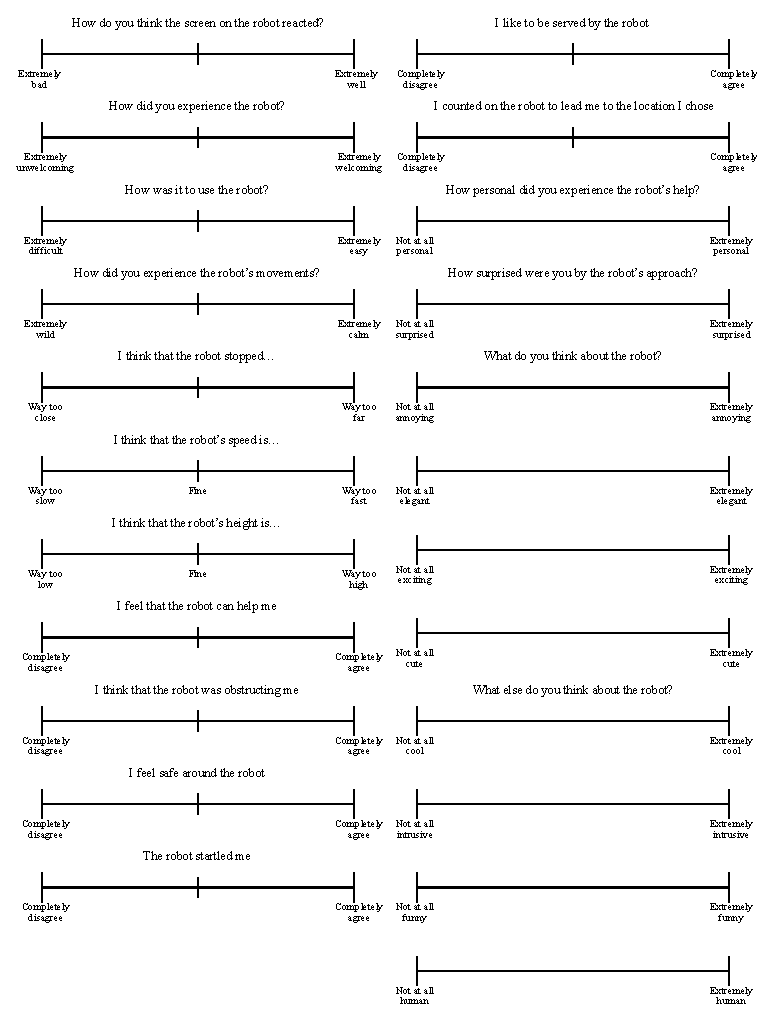
\includegraphics[width=1.0\linewidth]{AllScales.eps}
	%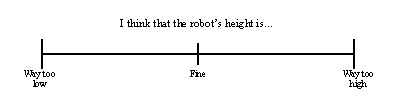
\includegraphics[width=0.4\linewidth]{RobotHeight.eps}
	%
\includegraphics[width=0.4\linewidth]{PersonalHelp.eps}
	%
\includegraphics[width=0.4\linewidth]{PersonalHelp.eps}
	%
\includegraphics[width=0.4\linewidth]{PersonalHelp.eps}
	%
\includegraphics[width=0.4\linewidth]{PersonalHelp.eps}
	%
\includegraphics[width=0.4\linewidth]{PersonalHelp.eps}
	%
\includegraphics[width=0.4\linewidth]{PersonalHelp.eps}
	%
\includegraphics[width=0.4\linewidth]{PersonalHelp.eps}
	%
\includegraphics[width=0.4\linewidth]{PersonalHelp.eps}
	%
\includegraphics[width=0.4\linewidth]{PersonalHelp.eps}
	%
\includegraphics[width=0.4\linewidth]{PersonalHelp.eps}
	%
\includegraphics[width=0.4\linewidth]{PersonalHelp.eps}
	%
\includegraphics[width=0.4\linewidth]{PersonalHelp.eps}
	%
\includegraphics[width=0.4\linewidth]{PersonalHelp.eps}
	%
\includegraphics[width=0.4\linewidth]{PersonalHelp.eps}
	%
\includegraphics[width=0.4\linewidth]{PersonalHelp.eps}
	%
\includegraphics[width=0.4\linewidth]{PersonalHelp.eps}
	%
\includegraphics[width=0.4\linewidth]{PersonalHelp.eps}
	%
\includegraphics[width=0.4\linewidth]{PersonalHelp.eps}
	%
\includegraphics[width=0.4\linewidth]{PersonalHelp.eps}
	%
\includegraphics[width=0.4\linewidth]{PersonalHelp.eps}
	%
\includegraphics[width=0.4\linewidth]{PersonalHelp.eps}

%	\textbf{Figure~2. }The three types of VAS developed from the elicitated variables.
\end{center}
%\vspace{-10pt}
}



\headerbox{Results - Scale Testing}
{name=results2,span=1,column=2,aligned=introduction}
{\parskip 5pt


}


\headerbox{Conclusion}
{name=conclusion,span=1,column=3,aligned=introduction}
{\parskip 5pt
This research conducted in this study reveals that there are at least 23 variables that danish travellers find important when interaction with a social robot. 


}


\headerbox{Acknowledgements}
{name=akn,span=1,column=3,below=conclusion}
{\parskip 5pt

}


\headerbox{Key references}
{name=references,column=3,below=akn}
{
\renewcommand{\section}[2]{}%
%\parskip 5pt
 %   \bibliography{bib.bib}
%\tiny
\footnotesize
%Dorte har skrevet kilder ind på følgende måde
%Abdala C (1996) JASA \textbf{100}(6):3726-3740.
%Bonfils P et al. (1991) \textit{Arch Otolaryngol Head Neck Surg} \textbf{117}(10):1167–1171.
%Brown DK et al. (2000) \textit{Hearing Res}. \textbf{145}(1-2):17-24.
}


%-------------------------------------------------------------------------

\end{poster}
\end{document}